%==================================================================================================
%   LUKES THESIS TEMPLATE 1.2
%   -------------------------
%   This template is based upon the offcial IMM PhD Thesis template, it is enhanced with a number
%   of new features and a number of errors have fixed. This template is intended to be complied to
%   PDF using PDFLATEX and is tested using the MiKTeX 2.9 LaTeX distribution.
%   It is based on the official DTU-IMM Thesis template by Finn Kuno Christensen in 2009.
%   Small bugfixes by Kasper Laursen in 2012 and 2013.
%   Small updates by Finn Kuno Christensen/Henning Christiansen in 2015.
%   -------------------------
%   Last Updated: 2015-01-08
%==================================================================================================
%
%==================================================================================================
% DOCUMENT SETUP
%==================================================================================================
\documentclass[10pt,twoside]{book}                  %Official DTU-IMM Thesis document setup
%
%Set to 'print' for printed version, use 'net' for online version
\def\thesisversion{print}
%
%==================================================================================================
% PACKAGES
%==================================================================================================
\usepackage{LukeThesis}                             %Import Thesis base style
%input{PhDMacros}                                   %Thesis specific macros
%
%==================================================================================================
% THESIS PROPERTIES (Modifiy these fields with your details)
%==================================================================================================
\def\thesisauthor{Jonathan Becktor and Christian Kiær}                     %Author
\def\thesistitle{TMTO Attack on the 3G Block Cipher Kasumi}               %Title
\def\thesishandin{25-June}                       %Submission date (Day-Month}
\def\thesisdegree{B.Sc.}                              %Degree ('B.Eng', 'B.Sc.', 'M.Sc.' or 'PhD')
\def\thesisyear{2015}                               %Submission year
\def\thesisnumber{????}                             %DTU-IMM Serial number (do not include year)
\def\thesisISSN{0000-0000}                          %ISSN number
\def\thesiskeywords{Keywords are, comma separated}  %PDF keywords
\derivethesisprops                                  %Derive dependent properties
%
%==================================================================================================
% SECTION NUMBERING SETUP
%==================================================================================================
\setcounter{tocdepth}{2}                            %2 adds sections up to subsections
\setcounter{secnumdepth}{3}                         %Subsubsections get a number when this is 3
%
%==================================================================================================
% THESIS STRUCTURE  (Modifiy to include more chapters etc)
%==================================================================================================
\begin{document}
%------------------------
%Pre-frontmatter material
%------------------------
\prefrontmatter
%--------------------
%Frontmatter material
%--------------------
\frontmatter
\pagenumbering{roman}                               %Set frontmatter numbering style
\chapter{Summary (English)}

The goal of the thesis is to ...                                   %English summary of Thesis
\markboth{}{}                                       %Set headings (left)(right)
\chapter{Summary (Danish)}
\begin{otherlanguage}{danish}

Målet for denne afhandling er at udføre et time-memory trade-off
angreb på KASUMI krypteringsalgoritmen som bruges i GSM.

KASUMI krypteringsalgoritmen bliver brugt til kryptering af data i the
Global System of Mobile Communications (GSM), specifikt i 2G og 3G
iterationerne.

For at udføre et time-memory trade-off angreb må vi først overveje
de forskellige udgaver af TMTO angrebet. I denne afhandling vil vi
kigge på de mest almindelige trade-off angreb, navnligt Hellman
trade-off, DP trade-off og Rainbow trade-off. Beregninger for de 3
typer af angreb er blevet lavet, med KASUMI angrebet i tankerne. Vi
fandt at rainbow angrebet er det mest effektive angreb, når der tænkes
på KASUMI.

Vi kan konkludere at et time-memory trade-off angreb er muligt på
KASUMI, men at den lange pre-beregningsmæssige process vil være en
stor forhindring. Modifikationer til vores implementation er også
nødvændige for at gøre angrebet mere muligt. Omkostningerne ved
udførsel af angrebet har vist sig at være relativt høje.

\end{otherlanguage}

%%% Local Variables:
%%% mode: latex
%%% TeX-master: "Thesis"
%%% End:
                                   %Danish summary of Thesis
\markboth{}{}                                       %Set headings (left)(right)
\chapter{Preface}

% % % EOF % % %
                                     %Preface
\markboth{}{}                                       %Set headings (left)(right)
\chapter{Acknowledgements}


We wish to express our sincere thanks to Dr. Andrey Bogdanov,
Associate Professor, for accepting our project and guiding us through
the whole project providing us with the means to complete this thesis.

We would also like to express much graditute towards Stefan Koebl,
Ph.D Student in the Cryptology group, for always providing guidance
and help throughout the project.


%%% Local Variables:
%%% mode: latex
%%% TeX-master: "Thesis"
%%% End:

                            %Acknowledgements
\markboth{}{}                                       %Set headings (left)(right)
%------------------
% Table of contents
%------------------
\newpage\mbox{}\newpage
\chaptermark{Contents}
\pdfbookmark{\contentsname}{toc}
\renewcommand{\sectionmark}[1]{\markright{#1}}
\sectionmark{Contents}
\addtolength{\parskip}{-\baselineskip}
\tableofcontents
\addtolength{\parskip}{\baselineskip}
\renewcommand{\sectionmark}[1]{\markright{\thesection\ #1}}
%-------------
% Main content
%-------------
\mainmatter
\chapter{Introduction}

\section{KASUMI Cipher and 2G/3G}

In this project, we analyse the real-world security of KASUMI as used
in 2G and 3G networks in form of A5/3 towards time-memory trade-off
attacks. KASUMI is a block cipher algorithm used in mobile embedded
systems to provide security between the phone and the base station. As
GSM is the international standard for mobile communication, KASUMI
is subject to a lot of cryptanalysis.

\section{TMTO Attack}

We will discuss some of the most popular time-memory trade-offs, give
the background theory behind them and try and analyze the best
TMTO-attack to use with KASUMI in mind.

The chosen TMTO-attack will be analyzed and optimal parameters for an
actual attack will be discussed.


\section{The problem}

The project will require an optimized implementation of the KASUMI
block cipher as described in papers. With the KASUMI cipher
implemented, the TMTO attack can be implemented

As the KASUMI cipher uses a keys with the size of \code{64-bit}, we
will have trouble testing an attack with hardware at our disposal. As
a solution we will implement an experimental attack using a key with
size \code{32-bit}. The experimental attack will allow us to generate
test results and provide us with the possibility of estimating how the
attack on a full keysize would operate.

Knowing some of the previous attacks performed on KASUMI, we can in
the conclusion conclude whether or not this attack can be seen as practical.

\section{Structure of the Thesis}

The thesis is structured such that we will first go through the theory
behind the KASUMI cipher (chapter \ref{ch:kas}) and the different TMTO
attacks (chapter \ref{ch:tmto}). We will proceed to look into the
actual table and parameter choices for the TMTO-attack (chapter
\ref{ch:param}). We will then go in depth with the
implementation of both KASUMI and the TMTO route we took(chapter
\ref{ch:impl}). Next we will analyze the results of the attack
(chapter \ref{ch:anal}). Afterwards we will move on to a discussion
about what further improvements could be made (chapter
\ref{ch:disc}). Finally we will give a conclusion of the project
(chapter \ref{ch:concl}).

%%% Local Variables:
%%% mode: latex
%%% TeX-master: "Thesis"
%%% End:
                                  %Chapter 1
\chapter{Theory}

\section{Kasumi}

The KASUMI block cipher is used in the GSM 
\subsection{Key schedule}
The keyschedule of the Kasumi cipher calculates all of the round keys,
from the given input key. The 128-bit key is split into eight 16-bit
subkeys, where $K_1,..K_8$ is a concatenation of subsequent 16-bit of
the original 128-bit key $K$.
\[K = K_1 || K_2 || K_3 || K_4 || K_5 || K_6 || K_7 || K_8\]
A modified key $K'$ is also generated by XOR'ing the original key with
the number $0x123456789ABCDEFFEDCBA9876543210$. This key $K'$ is split
into eight 16-bit subkeys as well, following the same rules of the
original key.
\[K' = K'_1 || K'_2 || K'_3 || K'_4 || K'_5 || K'_6 || K'_7 || K'_8\]
Thereafter eight round keys are generated as follows:
\begin{align*}
  KLi1 &= ROL16(K_i,1)\\
  KLi2 &= K'_{i+2}\\
  KOi1 &= ROL16(K_{i + 1},5)\\
  KOi2 &= ROL16(K_{i + 5},8)\\
  KOi3 &= ROL16(K_{i + 6},13)\\
  KIi1 &= K'_{i+4}\\
  KIi2 &= K'_{i+3}\\
  KIi3 &= K'_{i+7}\\
\end{align*}

\subsection{Algorithm}
The Kasumi algorithm takes an 64-bit word as an input. This word is
split into two halves.
\[ inputword = R_o || L_o\]
In each round of the algorithm the right half of the input is XOR'ed
with the output of the round functions. Thereafter the right and left
values are swapped. 
\begin{align*}
  L_i &= F_i(KL_i,KO_i,KI_i,L_{i - 1}) \oplus R_{i - 1} \\
  R_i &= L_{i - 1}
\end{align*}
Where $i$ determines which round function is used. A different round
function is used for odd and even rounds of the algorithm.

An odd round consists of the following:
\[F_{i = odd} = FO(KO_i, KI_i, FL(KL_i, L_{i - 1})) \]
Whereas an even round is performed as follows:
\[F_{i = even} = FL(KL_i, FO(KO_i,KI_i, L_{i - 1})) \]
After the last round the output ciphertext is the concatenation of the
outputs.
\[cipher = R_8 || L_8\]

#TODO
FL OG FO OG FI

\section{TMTO-Attack}



\subsection{Hellman Tables}

\subsection{Distinguished Points Tables}

\subsection{Rainbow Tables}

%%% Local Variables:
%%% mode: latex
%%% TeX-master: "Thesis"
%%% End:

\chapter{Implementation}
\section{KASUMI Cipher}
\subsection{Implementation}
The implemenation of the KASUMI follows the theory described in the
chapter \nameref{ch:kas}.


\subsection{Benchmarks and Performance}
The benchmarks of the KASUMI cipher implemented is performed on two
laptops. The Laptops will each compute the encryption on 64-bit of
data 10.000.000 times. An average time of ten runs of this test is
chosen as the result. Both machines run on Intels Hashwell
architecture with Core i7 CPUs. The specifications of the laptops are as follows:
\begin{table}[h!]
    \begin{tabular}{l|l|l}
                                    & Zenbook - i7           & Yoga
                                                               pro 2 -
      i7\\ \hline
    CPU Frequency                   & 1,8 GHZ @ 2.9ghz TURBO & 2,0 GHZ @ 3.0ghz TURBO \\ \hline
    CPU Cycles/s                    & 2900000000             & 3000000000             \\ \hline
    Times encryption of 64 bit data & 10000000               & 10000000               \\ \hline
    Total bit encyrpted             & 640000000              & 640000000              \\
    \end{tabular}
    \caption{CPU Specs of laptops performing benchmarks}
    \label{tab:specs}
\end{table}\\
The tests will be performed with the
GCC-compiler \footnote{The Gnu Compiler Collection -
  https://gcc.gnu.org/}. They will be performed with different compile
flags for optimization, consisting of no flags, O2, O3 and Ofast as
these are the most common flags for optimization. The two tables
\ref{tab:zen} and \ref{tab:yoga} will show the results of the KASUMI
tests.
\begin{table}[h!]
    \begin{tabular}{l|l|l|l|l}
     Zenbook 1.8 ghz.  & ~                     & ~             & ~              & ~               \\
    GCC compile flags. & Time in sec (average) & Cycles in tot & Cycles per bit & Cycles per byte \\ \hline
    None               & 7,2322                & 20973380000   & 32,77090625    & 262,16725       \\ \hline
    O2                 & 2,0035                & 5810150000    & 9,078359375    & 72,626875       \\ \hline
    O3                 & 1,8945                & 5494050000    & 8,584453125    & 68,675625       \\ \hline
    Ofast              & 1,897                 & 5501300000    & 8,59578125     & 68,76625        \\
    \end{tabular}
    \caption{Zenbook i7 benchmarks}
    \label{tab:zen}
\end{table}
\begin{table}[h!]
    \begin{tabular}{l|l|l|l|l}
     Yoga 2 pro 2.0 ghz. & ~                     & ~             & ~              & ~               \\
    GCC compile flags.   & Time in sec (average) & Cycles in tot & Cycles per bit & Cycles per byte \\ \hline
    None                 & 6,885                 & 20655000000   & 32,2734375     & 258,1875        \\ \hline
    O2                   & 1,933636364           & 5800909091    & 9,063920455    & 72,51136364     \\ \hline
    O3                   & 1,823333333           & 5470000000    & 8,546875       & 68,375          \\ \hline
    Ofast                & 1,835                 & 5505000000    & 8,6015625      & 68,8125         \\
    \end{tabular}
    \caption{Yoga 2 i7 benchmarks}
    \label{tab:yoga}
\end{table}\\


For analysis of the performance of the cipher, gprof \footnote{GNU
  Profiler - https://sourceware.org/binutils/docs/gprof/} is used to
analyze each function and get a clear idea of which functions might
cause slowdowns. The following output is produced from running the
tests and analyzing with gprof:
\begin{lstlisting}[caption=Gprof output,captionpos=b,label=lst:grpof]
    %   cumulative   self              self     total           
 time   seconds   seconds    calls  ns/call  ns/call  name    
 38.56      0.53     0.53 240000024     2.20     2.20  fi
 23.50      0.85     0.32                             keyschedule
 18.36      1.10     0.25 80000008     3.14     9.75  fo
 12.49      1.27     0.17 80000008     2.14     2.14  fl
  4.41      1.33     0.06                             kasumi_enc
\end{lstlisting}
Note that for getting an somewhat accurate representation of the time usage of
each function, the functions of the cipher cannot be inlined. Thus the
attribute \textit{noinline} must be included for each function. This
takes away some of the optimzations done by the Ofast compile
flag. Not supringsingly it shows that \textit{fi} and
\textit{keyschedule} takes up the most computational
power. Since \textit{fi} is used in every round of the cipher and it
requires lookups in a predefined table for every computation, this
could be seen as expected. As for the keyschedule, it's recalculated
in each encryption and therefore will require a new computation in
each new encryption done. 

If we consider the results of \ref{lst:grpof} and look at both
\ref{tab:zen} and \ref{tab:yoga}, this shows us that for each byte
encrypted around 17 cycles of the CPU is used on generating the
keyschedule. That leaves around 50 cylces remaining for the actual
encryption of a text.

Since most of the actual computations TODO assembly vs C? Find kilder?

Further optimization could be gained by using a different compiler. As
both test machines contain Intels i7 CPUs, noticeable performance
increases could be gained by using a Intel compiler. Tests with the
Intel compiler has not been performed. Kilder?

\section{Tablegenerator}

\section{Online Phase}

\section{Usage}


%%% Local Variables:
%%% mode: latex
%%% TeX-master: "Thesis"
%%% End:

\chapter{Analysis}
\label{ch:anal}

\section{TMTO Attack}
As the keysize of an attack on the KASUMI cipher used in the 2G
network is \code{64-bit}, we have to perform our tests on a scaled down
key. With the hardware at our disposal the computation of a table
required to perform the attack on a \code{64-bit} key would simply be
unrealistic. Therefore all of our testing is done on tables generated
with \code{32-bit} keys. We use the same idea as the scaling from \code{128-bit} to
\code{64-bit} discussed in chapter \ref{ch:kas}.

Thus a key $K$ built from a \code{32-bit} $K_{32} = K_1 || K_2$  implementation will
look as follows
\[K = K_1 || K_2 || K_1 || K_2 || K_1 || K_2 || K_1 || K_2\]
As to gain an idea of how our implementation matches up with
the math and parameter choices done in chapter \ref{ch:param}, we have to generate
information on an actual attack on a \code{32-bit} key. If the \code{32-bit} test
results match with our calculations, we can begin to give estimates
on the actual attack(\code{64-bit} keysize).
\subsection{Pre-computational phase}
To test the table generation we will first set some parameters
valid for \code{32-bit} testing.

Using the same parameter setup as described in \ref{sec:rainbowparam}
table \ref{tab:rainparam32} gives us valid parameter choices. For the
testing of \code{32-bit} no boundaries were set.
\begin{table}[H]
  \centering
  \text{\texttt{Success{ }={ }0.730000,{ }Rmsc{ }={ }1.849002,{ }l{ }={ }1,{ }Offline{ }phase{ }={ }2{\char`\^}32.886747}}
  \begin{tabular}{llll}
    m & t & M(MB) & T \\ \hline
    $2^{25.00}$ & $2^{7.89}$ & $134.22$ & $2^{13.67}$ \\
    $2^{25.50}$ & $2^{7.39}$ & $189.81$ & $2^{12.71}$ \\
    $2^{26.00}$ & $2^{6.89}$ & $268.44$ & $2^{11.76}$ \\
    $2^{26.50}$ & $2^{6.39}$ & $379.63$ & $2^{10.83}$ \\
    $2^{27.00}$ & $2^{5.89}$ & $536.87$ & $2^{9.92}$ \\
  \end{tabular}
  \caption{Rainbow Parameters - 32-bit keysize}
  \label{tab:rainparam32}
\end{table}
Since we are only testing on \code{32-bit} there is no real concern of
memory usage or online time. For this reason we went with a parameter
choice of $m=2^{25} \approx 33445532$ and $t= 2^{7.89} \approx
236$. The table generator will be tested on the actual
pre-computational time and the memory usage.

\textbf{Pre-computational time}

Table \ref{tab:rainparam32} states that an expected amount of
KASUMI encryptions required for generation of the table is
$2^{32.886}$. Looking back to \ref{sec:benchkas} we know the
amount of time it takes our test machines to perform 10000000 encrytions. As an
example the previously mentioned Zenbook i7 is used. The
Zenbook will perform 10000000 KASUMI encryptions in 1,897
seconds. From this we get an idea of how many encryptions our
machine execute in 1 second.
\[10000000 enc / 1.897 s = 5291005,29 \quad enc/s\]
Now we can calculate the expected running time of the
pre-computational phase
\[2^{32.886} / 5291005.29 \approx 1500s = 25 min \]
Running our implementation with UNIX-command
\code{time}\footnote{\url{https://en.wikipedia.org/wiki/Time_(Unix)}}
allows us to easily check whether or not this matches up. Running the
implementation multiple times resulted in average running time of
approximately 27 minutes. This is $\approx8\%$ more time used than
expected. This can be seen as expected as time is required to write
the table to a disk. Another explanation could be our sequential
approach and the usage of the MD5 algorithm. TODO Some facts to back up maybe?

\textbf{Memory}

We also want to make sure that the actual memory usage matches up with
the expected. From our parameter choice we can see the expected memory
$M_{predicted}=134.22$MB. The previously generated table can easily be
checked to make sure this is correct. Using the UNIX-command
\code{wc}\footnote{\url{https://en.wikipedia.org/wiki/Wc_(Unix)}} with
the \code{-c} flag will allow us to get the byte count of the
generated binary file. Performing this command on our generated table
unsurprisingly gave us a result of
$M_{actual}=134217728\text{B}\approx134.22$MB.

Knowing the time usage and memory usage in the pre-computational phase
matches up with our expected values, we can now give an approximate of
how scaling from a \code{32-bit} keysize to a \code{64-bit} keysize
will look.

Again we take a look back to \ref{sec:rainbowparam}. As we are now
dealing with the actual \code{64-bit} attack the boundaries we set
will now be taken into account again. From the tests on the
\code{32-bit} implementation we saw the size of the table match up
perfectly. Because of this we will not discuss table size further, as
adding additional bit to a binary file should not change the outcome.
Going with the parameters chosen in \ref{sec:rainbowparam} we set
$m=?$ and $t=?$.

From the chosen parameters we know that the pre-computational phase is
estimated to require $2^{64.88}$ encryptions of KASUMI. This amount of encryptions
is infeasible to test on the devices that we ran the
\code{32-bit} implementation on.

TODO Need to ask Andrey about what we can compare with.. HPC clusters?

\subsection{Online phase}
As stated earlier are the tests preformed on a scaled down version of the keyspace.
The tests are run on the 32 bit implementation and then scaled up.
Firstly the Time it takes is compared to our computations, as Time is found by $Time=\frac{t\cdot(t-1)}{2}$.
Table\ref{tab:OnlineT} shows each of our test tables worst case run times and the calculated encryption time for each of them.
Each  table has an online encryption time spanning from a few miliseconds to a few microseconds, wheras the total time is  much larger.
Furthermore if we don't add in the fact that the computer is smart and caches memory it takes even longer, which is shown in the T lookup field(this the time one lookup takes when it isn't in memory multiplied with t which is the amount of lookups).
\begin{table}[H]
\centering
\caption{Online Time Comparison}
\label{tab:OnlineT}
\begin{tabular}{|c|ccccc}
\hline
Table          & \multicolumn{1}{c|}{t rounded up} & \multicolumn{1}{c|}{Total time} & \multicolumn{1}{c|}{T lookup} & \multicolumn{1}{c|}{T enc} & \multicolumn{1}{c|}{encryptions} \\ \hline
134MB / 73\%   & 236                           & 7.5995 s                        & 7.972375 s                    & 5.24E-03 s                 & 27,730.00                        \\ \cline{1-1}
4300MB / 73\%  & 8                             & 27.339 s                        & 36.724 s                      & 5.29E-06 s                 & 28.00                            \\ \cline{1-1}
8500MB / 73\%  & 4                             & 73.35 s                         & 67.196 s                      & 1.13E-06 s                 & 6.00                             \\ \cline{1-1}
12000MB / 73\% & 3                             & 70.97 s                         & 69.811 s                      & 5.67E-07 s                 & 3.00                             \\ \cline{1-1}
17000MB / 73\%  & 2                             & 66.96 s                         & 65.11 s                       & 1.89E-07 s                 & 1.00                             \\ \cline{1-1}
\end{tabular}
\end{table}
This means that the biggest bottleneck in the implementation is the lookup time. To further investigate this we calculate the lookup time for each table, and compare them to each other note that the test computer has a max read speed of 540 mb/s. One thing we noticed is when the entire table can fit in memory the access time of it increases dramatically, for the 4.3GB table the first table lookup took 4.4 seconds and the lookups afterwards took between 0.6-1 seconds. This is probably due to the table getting cached.
\begin{table}[h]
\centering
\caption{Access time}
\label{tab:memory}
\begin{tabular}{|c|clccc}
\hline
\multicolumn{1}{|l|}{Buffer-size$\downarrow$ Table-size$\rightarrow$}& \multicolumn{1}{c|}{134MB} & \multicolumn{1}{l|}{4300MB} & \multicolumn{1}{c|}{8500MB} & \multicolumn{1}{c|}{12000MB} & \multicolumn{1}{l|}{17000MB} \\ \hline
33554432                                     & 0.0427s                    & 4.4395s                     & 16.829s                     & 23.230s                      & 32.562s                      \\ \cline{1-1}
524288                                       & 0.023s                     & 4.4395s                     & 16.645s                     & 23.279s                      & 32.72s                       \\ \cline{1-1}
65536                                        & 0.021s                     & 4.4585s                     & 16.941s                     & 23.002s                      & 32.483s                      \\ \cline{1-1}
32                                           & 0.053s                     & 5.0245s                     & 16.780s                     & 23.57s                       & 32.44s                       \\ \cline{1-1}
\multicolumn{1}{|l|}{Scaled to 8 tb table}   & 0.6 Hours                  & 2.37 Hours                  & 4.45 Hours                   & 4.31 Hours                   & 4.25 Hours                   \\ \cline{1-1}
\end{tabular}
\end{table}
As \ref{fig:memory} shows the buffer size does not seem to matter much the results fluxuates half a second at most.
The table also shows what the lookup time would be if the table was 8 tb. Where target table size is tts, table size is ts, s is the time one lookup takes in seconds and 3600 is to get it in hours $\frac{\frac{tts}{ts/s}}{3600}$
\begin{figure}[th]
  \centering
  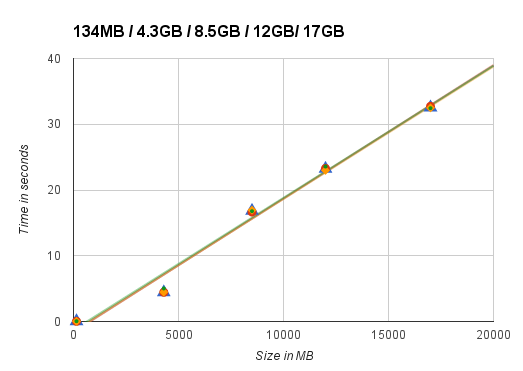
\includegraphics[width=0.8\textwidth]{figures/AccessTime.png}
  \caption{Access time for different table sizes and buffer sizes\\
    Green buffersize= 33554432 bit\\
    Red buffersize = 524288 bit\\
    Orange buffersize = 65536 bit\\
    Blue buffersize = 32 bit\\
    }
  \label{fig:tableAccess}
\end{figure}

Also something to note when scaling the access time up to a table that is 8tb the lookup time is around 4.2-4.45 hours.
One thing to note though is when the table is small enough to fit the memory it gives faster results, which can be ignored since the entire 8 tb table does not fit memory. Now where the access time is estimated we can give a approximation of the online phase for the \code{64-bit} keyspace. As previously stated the access time would lie around 4.2-4.45 hours for each lookup, so for $m=2^{39.80}$ and $t=2^{25.08}$ this means that the lookup time comes to $t\cdot lookupTime=2^{25.08}\cdot 4.45 Hours \approx 18,005 years$. The Encryption time would be $2^{25.08}\cdot\frac{2^{25.08}-1}{2}\approx \frac{6.2897672e+14 encryptions}{5291005 encryptions/sec} \approx 3.7 years$ so the online phase would approximately take $18008.7 years$. Which leads to the conclusion that our implementation would not work in its current state. To get a more realistic attack we will in section \ref{sec:Discussion} explain some memory optimizations and the RainbowDP table that reduces the amount from t to 1. To get the encryption time down to approximately one day one would need 1280 cores.


\section{Cost analysis}
In this section we will assume that the memory optimizations has been implemented and the table is of Rainbow/DP\ref{sec:Discussion}. This gives a table access of 1, when a DP is reached.
To pull this off for $m=2^{39.80}$ and $t=2^{25.08}$ the pre-computation will require \code{7.56TB}, and \code{$2^{64.88}$} encryptions. The online phase will require \code{$2^{49.16}$} encryptions, our cost analysis will aim at getting the online phases encryption time down to one day. This will require $\frac{2^{49.16}}{60*60*24}\approx 2^{32.76}$ encryptions per second. We have found a couple of candidates that fits the bill:

% Please add the following required packages to your document preamble:
% \usepackage[table,xcdraw]{xcolor}
% If you use beamer only pass "xcolor=table" option, i.e. \documentclass[xcolor=table]{beamer}
\begin{table}[h]
\caption{Hardware comparison}
\label{my-label}
\begin{tabular}{|ccccccc}
\hline
\rowcolor[HTML]{EFEFEF}
CPU                                    &                             &                               &                           &                                 &                            & \multicolumn{1}{l|}{\cellcolor[HTML]{EFEFEF}} \\ \hline
\multicolumn{1}{|c|}{Model}            & \multicolumn{1}{c|}{Cores}   & \multicolumn{1}{c|}{Amount} & \multicolumn{1}{c|}{Ghz}  & \multicolumn{1}{c|}{Enc per sec} & \multicolumn{1}{c|}{Price USD} & \multicolumn{1}{c|}{Total USD}                    \\ \hline
\multicolumn{1}{|l|}{AMD FX-8320}      & 8                            & 143                         & 3,5                       & 7278941245                      & 139                    & 20020                                     \\
\multicolumn{1}{|l|}{AMD FX-8350}      & 8                            & 125                         & 4                         & 7271669575                      & 170                   & 21250                                    \\ \hline
\rowcolor[HTML]{EFEFEF}
Hard Drive                                                          &                               &                           &                                 &                           & & \multicolumn{1}{l|}{\cellcolor[HTML]{EFEFEF}} \\ \hline
\multicolumn{1}{|c|}{Model}            & \multicolumn{1}{c|}{Size GB} & \multicolumn{1}{c|}{Amount} & \multicolumn{1}{c|}{Read $mb/s$} & \multicolumn{1}{c|}{Write $mb/s$}      & \multicolumn{1}{c|}{Price USD} & \multicolumn{1}{c|}{Total USD}                    \\ \hline
\multicolumn{1}{|c|}{Crucial}          & 960                          & 8                           & 500                       & 400                             & 300                        & 2400                                          \\
\multicolumn{1}{|c|}{Mushkin} & 1000                         & 8                            & 560                       & 460                             & 339                        & 2712                                          \\ \cline{1-1}
\end{tabular}
\end{table}
So with around $20020+2712=22732 $USD $ \approx 151313 $DK for the harddrive and the CPU's.

%%% Local Variables:
%%% mode: latex
%%% TeX-master: "Thesis"
%%% End:

\chapter{Discussion}
\label{ch:disc}
%%% Local Variables:
%%% mode: latex
%%% TeX-master: "Thesis"
%%% End:

\chapter{Conclusion}
\label{ch:concl}
A summary of the main part of the text
A deduction made on the basis of the main body
Your personal opinion on what has been discussed
A statement about the limitations of the work
A comment about the future based on what has been discussed
The implications of the work for future research

In this project we tried to analyze a practical attack on the KASUMI
block cipher by implementing a time-memory trade-off attack. We
conducted experiments to determine whether or not this attack can be
seen as practical. 

The biggest obstacle in performing this attack will undoubtedly be
computation of the tables needed for the attack. Generating such table
will require more than $2^{64}$ computations of KASUMI if a decent
success probability is expected.

Our implementation of the attack is also very unoptimized when
considering large tables consisting of multiple terabytes of
data. Read times and lookups in tables will prove to be a huge
hindrance if the attack is to be performed on the full keyspace of
\code{64-bit}.

If the attack is to be considered doable the combined approach of 
rainbow and DP attacks should definitely a part of the
implementation. 

%%% Local Variables:
%%% mode: latex
%%% TeX-master: "Thesis"
%%% End:

\appendix
\chapter{Appendix}
\section{Installation}
\label{sec:inst}
Get the source:

\quad\code{\$ git clone \url{https://github.com/kiaer/kasumi.git}}

Build the TMTO-attack. This will generate the executable
\code{bin/tmto}

\quad\code{\$ make }

The executable \code{tmto} can now be executed with an appropriate
flag:

\quad\code{\$ ./bin/tmto [command]}

The following commands is available to use with \code{tmto}:
\begin{verbatim}
usage: ./bin/tmto [command] 
                -t      Generates 32-bit Rainbow Table 
                -o      Performs online phase on 32-bit Rainbow Table 
                -b      Generates 64-bit Rainbow Table 
                -k      Performs online phase on 64-bit Rainbow Table 
                -h      Prints the very helpful usage message.. 
\end{verbatim}

Generating a table for either the 32-bit or the 64-bit key, the table
is stored in the kasumi root folder as either \code{table32.bin} or
\code{table64.bin}. The onlinephase will perform the attack on its
respective table.

Generation of the cipher, for test purposes is also possible:

\quad\code{\$ make cipher}

An executable \code{bin/kasumi\_test} is created. 

%%% Local Variables:
%%% mode: latex
%%% TeX-master: "Thesis"
%%% End:
                                 %Appendix A
%-----------
% Backmatter
%-----------
\backmatter
\chaptermark{Bibliography}
\renewcommand{\sectionmark}[1]{\markright{#1}}
\sectionmark{Bibliography}
\addcontentsline{toc}{chapter}{Bibliography}        %Force addition of Bibliography to TOC
\bibliographystyle{alpha}                           %Use alpha codes for references
\bibliography{References}                           %Bibliography file called
\end{document}
% % % EOF % % %
%%% Local Variables:
%%% mode: latex
%%% TeX-master: t
%%% End:
